\section{Precision of system}\label{sec:precisionofsystem}

This experiment will test the precision of the complete system. 

\subsection{Range}

The system will change between two different positions, and stop when it has reached as it best can. When controller stops the position are marked, and the other position is set to the controller which now converges to this position. When it reaches it the position are marked and it will begin moving to the former position etc. \dots This is done ten times.

\subsection{Test Setup}\label{subsec:testsetup}

The test is performed by fastening a laser pointer on the pan/tilt system. A board is placed next to the system and two positions were the pointer is on the board are chosen \ref{fig:systemtestsetup}. The laser pointer is placed 174 cm and 180.5 from each point. Thus each degree is at around 3 centimetres wide.

\[ \frac{\Pi*2*174}{360} = 3.03687 \]


\begin{figure}[htb]
	\centering
	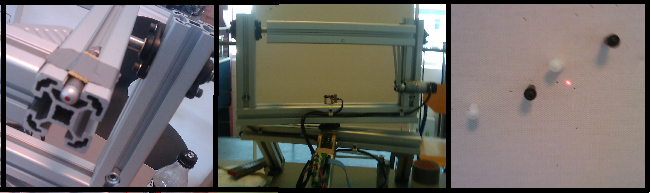
\includegraphics[scale=0.9,trim=0 0 0 0]{graphics/overallsystemtest.png} %trim=l b r t (can cut off from every side)
	\caption{Setup if the test. From left to right; the mounted laser, the system pointing at the board, laser dot and marks.}
	\label{fig:systemtestsetup}			% figure labels are of the form \label{fig:*}
\end{figure}


\subsection{Result}

At both points the error was less than five centimetres and at most of the time less than two. This means that the system have an uncertainty between 0.658 and 3.293 degrees. This precision is reached with overshoot.

\[ \frac{2.0}{3.03687} = 0.658 \]

\[ \frac{10.0}{3.03687} = 3.293 \]

\subsection{Conclusion}

The system itself, when no account is taking the elasticity, have a precision of af third degree.
\[ \frac{1080.0}{360} = 3 \]
It is a high precision that have been observed, at times the uncertainty is so small that it comes from uncertainty in the system. The system is though not able to hit the position without overshooting. But as precision and not speed was our objective this is a satisfying result, but it is also showing that better precision can be obtained.
